
\فصل{مسیریابی}
در هر شبکه‌ای، این مسیریاب‌ها هستند که بسته‌ها را به مقصد خود می‌رسانند. هر مسیریاب به تعدادی مسیریاب دیگر متصل است و مجموعه آن‌ها یک گراف را تشکل می‌دهند. هر مسیریاب باید بداند که بسته‌ای که به آن رسیده است را روی کدام واسط خود بفرستند. 
پروتکل مسیریابی مشخص می‌کند که مسیریاب‌ها چگونه با یکدیگر در ارتباط‌‌ هستند و اطلاعاتی را رد و بدل می‌کنند تا در نهایت بتوانند مسیری که یک بسته باید طی کند را مشخص کنند و بسته را در مسیر درست هدایت کنند. هر مسیریاب در ابتدا فقط اطلاعات پیوندهایی را دارد که به طور مستقیم به آنها متصل است و این وظیفه پروتکل مسیریابی است که یه نوعی اطلاعات لازم را به هر مسیریاب برساند تا او بتواند به ازای هربسته، مسیر درست را تشخیص دهد. 

پروتکل‌های مسیریابی به دو دسته اصلی تقسیم می‌شوند:‌

\شروع{فقرات}
\فقره پروتکل‌های مبتنی بر وضعیت پیوند\زیرنوشت{link-state protocols}، مانند OSPF\زیرنوشت{Open Shortest Path First}
و
 IS-IS
 \زیرنوشت{Intermediate System to Intermediate System}
\فقره پروتکل‌های مبتنی بر بردار فاصله\زیرنوشت{distance-vector protocols} مانند RIP\زیرنوشت{Routing Information Protocol}
و IGRP\زیرنوشت{Interior Gateway Routing Protocol}
\پایان{فقرات}
 در ادامه به توضیح مختصری راجع به این دو مدل مسیریابی می‌پردازیم:
 
 \قسمت{پروتکل مبتنی بر وضعیت پیوند}
 ایده اصلی پشت این پروتکل این است که هر مسیریاب یک نقشه کلی از گراف شبکه را در اختیار دارد و با توجه به آن، خودش کوتاهترین مسیر را محاسبه کند. محاسبه کوتاهترین مسیر به وسیله استفاده از الگوریتم دایسترا\زیرنوشت{Dijkstra's algorithm} صورت می‌پذیرد. در پروتکل وضعیت پیوند، هر مسیریاب وضعیت پیوند‌های خودش را می‌داند (‌اینکه آیا این پیوند هنوز برقرار است یا نه و اینکه هزینه ارسال از طریق این پیوند چقدر است ). و این اطلاعات را درون شبکه پخش\زیرنوشت{broadcast} می‌کند تا همه بتوانند یک دید کلی از گراف شبکه داشته باشند. هر مسیریاب بعد از آنکه اطلاعات همسایه خودش را گرفت، آن را به همه همسایگانش (‌به جز کسی که این بسته را از او دریافت کرده)‌ می‌فرستد و به این طریق اطلاعات این بسته در کل شبکه پخش می‌شود. (‌شکل 
~\ref{fig:linkstate}
 )
 \begin{figure}[H]
\centering
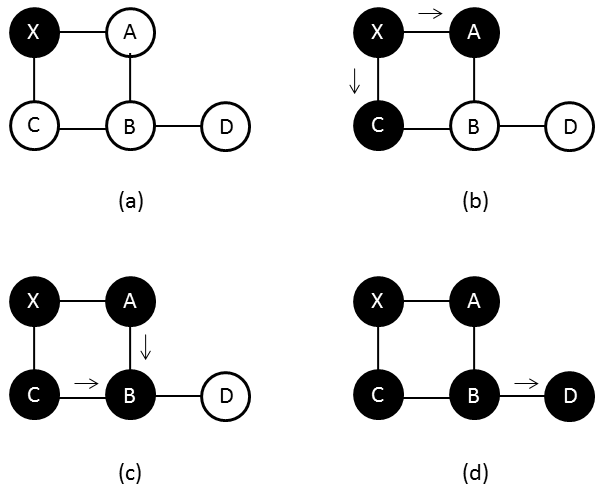
\includegraphics[scale=0.8]{./resources/figures/linkstate.png}
\caption{فرستاده شدن بسته‌‌های اطلاعات در پروتکل وضعیت پیوند}
\label{fig:linkstate}
\end{figure}
 
 مسیریاب‌ها برای آنکه از برقرار بودن پیوند میان خود و همسایگانشان اطمینان حاصل کنند، به طور متناوب بسته‌های سلام\زیرنوشت{}ای را به یکدیگر ارسال می‌کنند. اگر یک مسیریاب برای مدتی از یکی از واسط‌هایش پیام سلام را دریافت نکند، آن پیوند را غیرفعال در نظر می‌گیرد و از گراف خود حذف می‌کند. سپس شروع به فرستادن بسته‌های به‌روز رسانی می‌کند. 
 
فرستاده شدن این پیام‌های به‌روزرسانی به سه دلیل اتفاق می‌افتد: اول وقتی است که توپولوژی تغییر می‌کند، یعنی یک پیوند و یا یک گره از کار می‌افتد و یا ترمیم می‌شود. دوم، زمانی که یک تغییر در هزینه‌های مربوط به پیوند‌ها اتفاق می‌افتد. و در نهایت، مسیریاب‌ها به طور متناوبی این مثلا با دوره تناوب ۳۰ دقیقه این به روزرسانی را انجام می‌دهند تا همه همیشه وضعیت درست شبکه را داشته باشند.  

همان‌طور که گفته شد، مسیریاب‌ها بلافاصله بعد از خراب شدن یک پیوند، متوجه خرابی نمی‌شوند.  یک مسئله‌ی جالبی که می‌توان به آن اشاره کرد وقتی است که یک مسیریاب زودتر از بقیه غیرفعال بودن یک پیوند را تشخیص دهد. در این موقعیت، چون گراف مسیریاب‌ها با هم تفاوت می‌‌کند، ممکن است هرکدام از آنها برای یک بسته، کوتاهترین مسیر متفاوتی را محاسبه کنند، و حتی ممکن است که به تبع این اتفاق، بسته برای مدتی داخل یک حلقه بیفتد. ولی به محض اینکه همه مسیریاب‌ها به روزرسانی شدند، این بسته اگر هنوز زنده باشد، به مسیر درست هدایت خواهد شد. 
 
 \قسمت{پروتکل مبتنی بردار فاصله}
در این پروتکل همان‌طور که از نام آن مشخص است، هر مسیریاب یک بردار دارد که نشان می‌دهد که کوتاهترین فاصله‌‌اش از هر مسیریاب دیگر چقدر است و اینکه این کوتاهترین مسیر از طریق کدام پیوندش آغاز می‌شود. در واقع هر مسیریابی صبر می‌کند تا یک تغییر در پیوند‌هایش را شناسایی کند، سپس مسیرهای خودش را دوباره محاسبه می‌‌کند و اگر تغییری در بردارش به وجود آمده بود، بردار جدید را برای همسایگان خود می‌فرستد و همه همسایگان آن با توجه به بردار خودشان و اطلاعاتی که دریافت کرده‌اند، بردارشان را به روزرسانی می‌‌کنند و بردار به روز رسانی شده را برای همسایگان خود می‌فرستند. در نگاه کلی این روند، الگوریتم بلمن-فورد را پیاده‌سازی می‌‌کند. این الگوریتم به این صورت است که در مرحله اول همه مسیرهای به طول ۱ به صورت بهینه بین همه مشخص شده‌اند. در مرحله دوم، همه مسیرهای به طول ۲ و همین‌طور الی آخر. 
برای تبیین بهتر این موضوع، این روند را با معرفی نمادهایی توضیح می‌دهیم:‌

فرض کنید که $c(x,v)$ هزینه پیوند موجود بین $x$ و $v$ باشد. $D_{x}(y)$ هزینه رسیدن به $y$ با مبدا $x$ است. پس مسیریاب $x$ شامل یک بردار به صورت $D_{x}=[D_{x}(y):y\in N]$ است. گره $x$ بردار همسایه خود به اسم $v$  را دریافت می‌‌کند و بعد به طریق زیر بردار خود را به 
روزرسانی می‌کند. $$D_{x}(y) \leftarrow min{c(x,v) + D_{v}(y), D_{x}(y)} for each y \in N$$
بر اساس الگوریتم بلمن-فورد، این بردار به مرور زمان همگرا می‌شود. 
   
  در این الگوریتم، در صورتی که هزینه یک پیوند کاهش پیدا کند، همه مسیریاب‌ها به سرعت به روزرسانی می‌شوند. اصطلاحا گفته می‌شود که خبرهای خوب زود پخش می‌شوند. برای روشن شدن این موضوع مثال زیر را درنظر بگیرید:
  

 \begin{figure}[H]
\centering
\makebox[\textwidth][c]{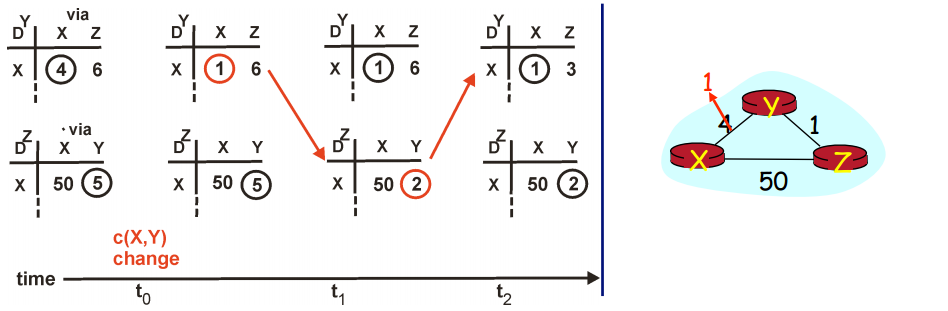
\includegraphics[width=1\textwidth]{./resources/figures/DV_goodnews.png}}
%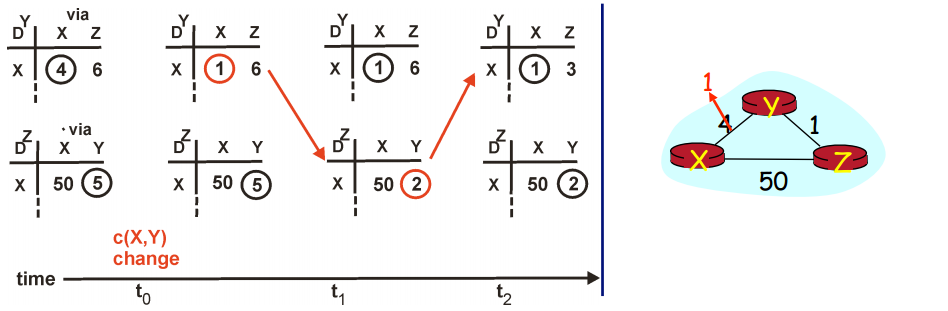
\includegraphics[scale=0.8]{./resources/figures/DV_goodnews.png}
\caption{کاهش هزینه یک پیوند و نحوه به روزرسانی‌شدن بردار‌های فاصله}
\label{fig:goodnews}
\end{figure}
 

 در شکل 
 ~\ref{fig:goodnews}
 هزینه پیوند بین $y$ و $x$ کاهش پیدا می‌کند. $y$ قبلا بهترین مسیرش به $x$ از طریق $x$ بوده و با هزینه‌ی ۴. اینک این هزینه به ۱ کاهش یافته است. در مرحله بعد $z$ که قبلا بهترین مسیرش به $x$ از طرف $y$ بوده، در این مرحله می‌بیند که فاصله‌اش تا $y$ ۱ است و $y$ هم که اعلام کرده تا $x$ ۱ است، پس طبق به‌روزرسانی‌ای که ذکر شد، $z$  مسیر خودش به $x$ را به ۲ کاهش می‌دهد و می‌آموزد که این مسیر از طریق $y$ است. 
 
 از طرف دیگر گفته می‌شود که طبق این الگوریتم، خبرهای بد دیر منتشر می‌شوند. در بیان دیگر به این مشکل، شمارش بی‌انتها\زیرنوشت{Count to Infinity Problem} هم گفته می‌شود. ماهیت این مشکل از جایی نشأت می‌گیرد که وقتی $x$ به $y$ می‌گوید که مسیری به جایی دارد، هیچ راهی برای $y$ وجود ندارد که بفهمد آیا خود $x$ جزو این مسیر است یا خیر. برای روشن شدن این موضوع مثال زیر را در نظر بگیرید: 
 
 \begin{figure}[H]
\centering
\makebox[\textwidth][c]{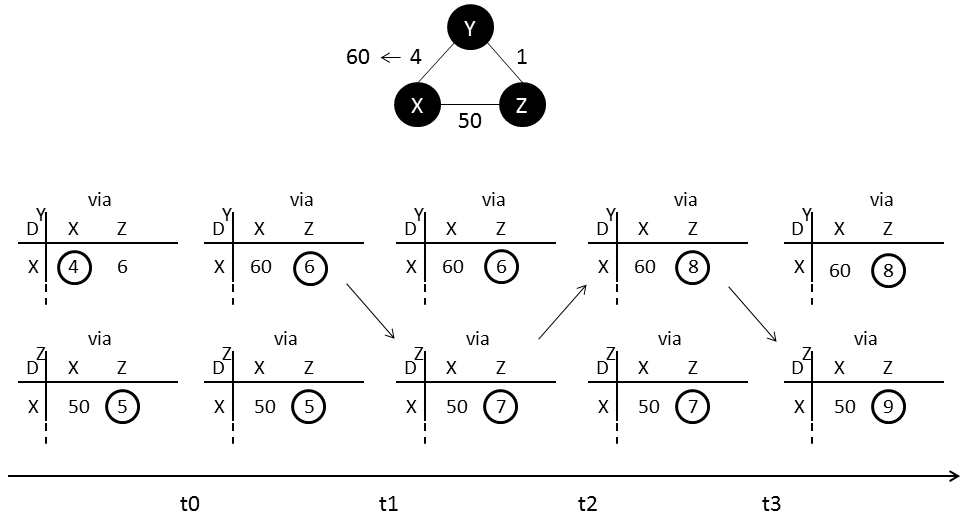
\includegraphics[width=1\textwidth]{./resources/figures/DV_badnews.png}}
\caption{افزایش هزینه یک پیوند و نحوه به روزرسانی‌شدن بردار‌های فاصله}
\label{fig:badnews}
\end{figure}
 
همان‌طور که در شکل 
~\ref{fig:badnews}
مشخص است، در ابتدا مسیر $y$ به $x$ از طریق $x$ با هزینه ۴ ، و از طریق $z$‌ با هزینه ۶ و با مسیر $y\Rightarrow z\Rightarrow y\Rightarrow x$   می‌باشد. در زمان $t_{0}$ ، هزینه پیوند بین $x$ و $y$ از ۴ به ۶۰ افزایش پیدا می‌کند. در مرحله بعد، $y$ هنوز فکر می‌کند که مسیر بهینه آن تا $x$ از طریق $z$ است و به هزینه ۶ و  $z$ که قبلا مسیر آن به $x$ از طریق $y$ بوده، این عنصر بردار خود را به هزینه $7$ افزایش می‌دهد. در مرحله بعد، به  $y$  اعلام شده است که مسیری به هزینه ۷ از طریق $z$ به  $x$وجود دارد. و بنابراین $y$ هزینه مسیر خود از طریق $z$ را به ۸ افزایش می‌دهد و این روند به همین ترتیب ادامه پیدا می‌کند و در هر مرحله هزینه مسیرها ۱ واحد افزایش پیدا می‌کند تا در نهایت به ۶۰ برسد. مشاهده می‌شود که روند همگرایی بسیار آرام بوده و به ویژه در زمانی که هزینه پیون افزایش زیادی پیدا کرده باشد، زمان رسیدن همه بردارها به مقدار درست، زیاد است و به همین دلیل نام شمارش بی‌انتها که برای این مشکل در نظر گرفته شده، بسیار مناسب است. 
